%\documentclass[
  bibliography=totoc,     % Literatur im Inhaltsverzeichnis
  captions=tableheading,  % Tabellenüberschriften
  titlepage=firstiscover, % Titelseite ist Deckblatt
]{scrartcl}

% Paket float verbessern
\usepackage{scrhack}

% Warnung, falls nochmal kompiliert werden muss
\usepackage[aux]{rerunfilecheck}

% unverzichtbare Mathe-Befehle
\usepackage{amsmath}
% viele Mathe-Symbole
\usepackage{amssymb}
% Erweiterungen für amsmath
\usepackage{mathtools}

% Fonteinstellungen
\usepackage{fontspec}
% Latin Modern Fonts werden automatisch geladen
% Alternativ zum Beispiel:
%\setromanfont{Libertinus Serif}
%\setsansfont{Libertinus Sans}
%\setmonofont{Libertinus Mono}

% Wenn man andere Schriftarten gesetzt hat,
% sollte man das Seiten-Layout neu berechnen lassen
\recalctypearea{}

% deutsche Spracheinstellungen
\usepackage[ngerman]{babel}


\usepackage[
  math-style=ISO,    % ┐
  bold-style=ISO,    % │
  sans-style=italic, % │ ISO-Standard folgen
  nabla=upright,     % │
  partial=upright,   % │
  mathrm=sym,        % ┘
  warnings-off={           % ┐
    mathtools-colon,       % │ unnötige Warnungen ausschalten
    mathtools-overbracket, % │
  },                       % ┘
]{unicode-math}

% traditionelle Fonts für Mathematik
\setmathfont{Latin Modern Math}
% Alternativ zum Beispiel:
%\setmathfont{Libertinus Math}

\setmathfont{XITS Math}[range={scr, bfscr}]
\setmathfont{XITS Math}[range={cal, bfcal}, StylisticSet=1]

% Zahlen und Einheiten
\usepackage[
  locale=DE,                   % deutsche Einstellungen
  separate-uncertainty=true,   % immer Unsicherheit mit \pm
  per-mode=symbol-or-fraction, % / in inline math, fraction in display math
]{siunitx}

% chemische Formeln
\usepackage[
  version=4,
  math-greek=default, % ┐ mit unicode-math zusammenarbeiten
  text-greek=default, % ┘
]{mhchem}

% richtige Anführungszeichen
\usepackage[autostyle]{csquotes}

% schöne Brüche im Text
\usepackage{xfrac}

% Standardplatzierung für Floats einstellen
\usepackage{float}
\floatplacement{figure}{htbp}
\floatplacement{table}{htbp}

% Floats innerhalb einer Section halten
\usepackage[
  section, % Floats innerhalb der Section halten
  below,   % unterhalb der Section aber auf der selben Seite ist ok
]{placeins}

% Seite drehen für breite Tabellen: landscape Umgebung
\usepackage{pdflscape}

% Captions schöner machen.
\usepackage[
  labelfont=bf,        % Tabelle x: Abbildung y: ist jetzt fett
  font=small,          % Schrift etwas kleiner als Dokument
  width=0.9\textwidth, % maximale Breite einer Caption schmaler
]{caption}
% subfigure, subtable, subref
\usepackage{subcaption}

% Grafiken können eingebunden werden
\usepackage{graphicx}

% schöne Tabellen
\usepackage{tabularray}
\UseTblrLibrary{booktabs, siunitx}

% Verbesserungen am Schriftbild
\usepackage{microtype}

% Literaturverzeichnis
\usepackage[
  backend=biber,
]{biblatex}
% Quellendatenbank
\addbibresource{lit.bib}
\addbibresource{programme.bib}

% Hyperlinks im Dokument
\usepackage[
  german,
  unicode,        % Unicode in PDF-Attributen erlauben
  pdfusetitle,    % Titel, Autoren und Datum als PDF-Attribute
  pdfcreator={},  % ┐ PDF-Attribute säubern
  pdfproducer={}, % ┘
]{hyperref}
% erweiterte Bookmarks im PDF
\usepackage{bookmark}

% Trennung von Wörtern mit Strichen
\usepackage[shortcuts]{extdash}

\author{%
  Vincent Wirsdörfer\\%
  \href{mailto:vincent.wirsdoerfer@udo.edu}{authorA@udo.edu}%
  \and%
  Joris Daus\\%
  \href{mailto:joris.daus@udo.edu}{authorB@udo.edu}%
}
\publishers{TU Dortmund – Fakultät Physik}


%\begin{document}
\section{Auswertung}
\label{sec:Auswertung}

Die Spannungamplitude der Referenzspannung kann variiert werden. Bei der Oszillatorspannung, also der Signalspannung, 
ist die Amplitude konstant und beträgt $U=3.2 \, \unit{\volt}$.\\

\subsection{Verifizierung der Funktionsweise eines Lock-In-Verstärkers}

Die im Lock-In-Verstärker gemischten Spannungen werden für die Phasenverschiebungen 
$\varphi= 0°,\, 90°,\, 180°,\, 270° \ \text{und} \ 315°$ abfotografiert. Die Phasenverschiebung $\varphi$ beschreibt dabei die 
Phase, welche zwischen der Referenz- und der Signalspannung liegt. Die Ausgangsspannung des Verstärkers besitzt bei den eben genannten Phasendifferenzen 
folgende Form:

\begin{figure}
    \begin{subfigure}{0.48\textwidth}
        \centering
        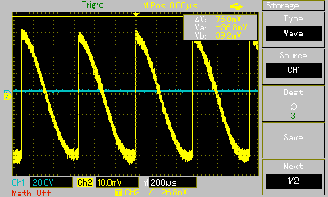
\includegraphics{./content/Oszilloskop_0.pdf}
        \caption{Phasenverschiebung $\varphi = 0°$.}
        \label{fig:0deg}
    \end{subfigure}
    \hfill
    \begin{subfigure}{0.48\textwidth}
        \centering
        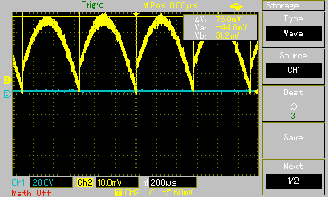
\includegraphics{./content/Oszilloskop_90.pdf}
        \caption{Phasenverschiebung $\varphi = 90°$.}
        \label{fig:90deg}
    \end{subfigure}
    \hfill
    \begin{subfigure}{0.48\textwidth}
        \centering
        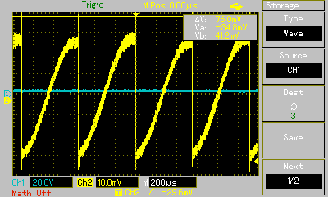
\includegraphics{./content/Oszilloskop_180.pdf}
        \caption{Phasenverschiebung $\varphi = 180°$.}
        \label{fig:180deg}
    \end{subfigure}
    \hfill
    \begin{subfigure}{0.48\textwidth}
        \centering
        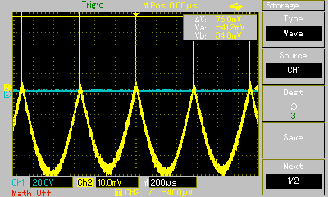
\includegraphics{./content/Oszilloskop_270.pdf}
        \caption{Phasenverschiebung $\varphi = 270°$.}
        \label{fig:270deg}
    \end{subfigure}
    \hfill
    \begin{subfigure}{0.48\textwidth}
        \centering
        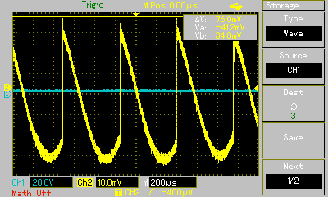
\includegraphics{./content/Oszilloskop_315.pdf}
        \caption{Phasenverschiebung $\varphi = 315°$.}
        \label{fig:315deg}
    \end{subfigure}    
\caption{Entwicklung der Ausgangsspannung $U_\text{Sig}$ in Abhängigkeit der Phase $\varphi$.}
\end{figure}

\noindent
Die Abbildungen, zwischen denen jeweils Phasenunterschiede von $180\,\unit{\degree}$ vorliegen (zum Beispiel $\varphi = 0\,\unit{\degree}$ und $\varphi = 180\,\unit{\degree}$), 
sind an der x-Achse gespiegelt. Dies kann dadurch begründet werden, dass die
Referenzspannung immer genau das gleiche beziehungsweise genau das entgegengesetzte Vorzeichen wie die 
Signalspannung besitzt. So hat zum Beispiel die Referenzspannung in \autoref{fig:90deg} das gleiche Vorzeichen wie die 
Signalspannung, weshalb nur positive Komponenten existieren. So haben in \autoref{fig:270deg} Referenz- und 
Signalspannung genau entgegengesetzte Vorzeichen.
Gleiches lässt sich auch bei \autoref{fig:0deg} und \autoref{fig:180deg} beobachten.\\\\
\noindent
Im folgenden werden die Messdaten aus \autoref{tab:no_noise} und \autoref{tab:mit_noise} ausgewertet. Die gemessene 
Spannung wird gegen die eingestellte Phasenverschiebung aufgetragen. Über ein Pythonprogramm wird zu der 
theoretisch vorhergesagten Funktion \eqref{eqn:U_out} eine Kurve gefittet.\\
Zunächst wird der phasenabhängige Amplitudenverlauf ohne externes Zuschalten eines Rauschsignals \emph{(Noise)} abgebildet.

\begin{figure}[H]
    \includegraphics[width=\textwidth]{no_noise.pdf}
    \caption{Nicht verrauschtes Signal.}
    \label{fig:fit_no_noise}
\end{figure}

\noindent
Gefittet wird hierbei eine cos-Funktion der Form:

\begin{equation*}
    A = a\cos(x - b) + c
\end{equation*}

\noindent Mittels der durch Python ausgegebenen Parameterwerte und der Gleichung \eqref{eqn:U_out} ergibt sich folgender Wert 
für die Amplitudenspannung:

\begin{equation*}
    U_0 = (0.522 \pm 0.015)\,\unit{\volt}
\end{equation*}

\noindent Nun wird durch den \emph{Noise Generator} ein zusätzliches Rauschsignal simuliert. Die folgende Abbildung zeigt den
dadurch entstehenden Amplitudenverlauf in Abhängigkeit der Phase.

\begin{figure}[H]
    \includegraphics[width=\textwidth]{mit_noise.pdf}
    \caption{Verrauschtes Signal.}
    \label{fig:fit_mit_noise}
\end{figure}

\noindent
Anhand der \autoref{fig:fit_mit_noise} lässt sich erkennen, dass die gemessenen Daten gut durch eine Kosinus-Funktion gefittet werden 
können. Auch wenn das Intervall der Phasenverschiebung im Vergleich zur \autoref{fig:fit_no_noise} nicht so gewählt 
wurde, dass eine komplette Periode abgedeckt wird, ist nichtsdestotrotz eine deutliche Elongation im Zetrum der Abbildung und 
andeutende Minima an den Rändern der Abbildung zu erkennen.\\
Analog zum Amplitudenverlauf ohne Rauschsignal lässt sich nun die Amplitudenspannung durch die von Python ausgegebenen Parameterwerte
und der Gleichung \eqref{eqn:U_out} bestimmen:

\begin{equation*}
    U_0 = (1.363 \pm 0.033)\,\unit{\volt}
\end{equation*}

\subsection{Rauschunterdrückung des Lock-In-Verstärkers durch einen Photodetektor}

Zur Überprüfung der Rauschunterdrückung des Lock-In-Verstärkers durch einen Photodetektor werden die Menge der Wertpaare
\{$x,U(x)$\} aus \autoref{tab:photonoise} graphisch aufgetragen. Die gemessenen Daten werden durch eine Funktion der Form

\begin{equation*}
    A = \frac{a}{x²} + b
\end{equation*}

\noindent gefittet. Dies lässt sich nun graphisch darstellen.

\begin{figure}
    \centering
    \includegraphics[width=\textwidth]{photodetektor.pdf}
    \caption{Intensitätsverlauf der LED in Abhängigkeit vom Abstand $x$.}
    \label{fig:photoabb}
\end{figure}

\noindent Die gefittete Kurve bestätigt den rapiden und asymptodischen Abfall der Intensität bei steigendem
Abstand $x$ zwischen LED und Photodiode.\\
Aufgrund der Beschädigung eines Reglers kann die Skalierung der Intensität nicht beliebig oft umgestellt weden. 
Dementsprechend wird der Abstand 

\begin{equation*}
    x_\text{max} = 90\,\unit{\centi\meter}
\end{equation*}

\noindent als letzter reliable Stelle ausgewertet\footnote{Eine intensivere Begründung folgt in der Diskussion.}.
%\end{document}
